\documentclass[11pt]{article}
\usepackage{fullpage,url,amssymb,epsfig,color,xspace,tikz,amsmath}
\usepackage{booktabs}
\usepackage{longtable}
\usepackage{graphicx}
\usepackage{makecell}
\usepackage{float}
\usepackage[pdftitle={CS 454 Assignment 1},
pdfsubject={University of Waterloo, CS 454, Winter 2024},
pdfauthor={Arne Storjohann}]{hyperref}
\usepackage{algpseudocode,enumitem,calc,multicol}



\usepackage{listings}
\lstset{%
        language=python,
        keepspaces=true,
        basicstyle=\small\ttfamily,
       commentstyle=\footnotesize\itshape{},
       identifierstyle=\slshape{},
       keywordstyle=\bfseries,
       numbers=left,
       numberstyle=\tiny{},
       numberblanklines=false,
       inputencoding={utf8},
       columns=fullflexible,
       basewidth=.5em,
        fontadjust=true,
        tabsize=3,
        emptylines=*1,
       breaklines,
       breakindent=30pt,
        prebreak=\smash{\raisebox{-.5ex}{\hbox{\tiny$\hookleftarrow$}}},
    escapeinside={//*}{\^^M} % Allow to set labels and the like in comments starting with //*
	}

\renewcommand{\thesubsection}{Question \arabic{subsection}}

\begin{document}

\begin{center}
  {\Large\bf University of Waterloo}\\ \vspace{3mm}
  {\Large\bf CS 454, Winter 2024}\\ \vspace{2mm}
  {\Large\bf Assignment 1}\\ \vspace{3mm}
\end{center}

\definecolor{care}{rgb}{0,0,0}
\def\question#1{\item[\bf #1.]}
\def\part#1{\item[\bf #1)]}
\newcommand{\pc}[1]{\mbox{\textbf{#1}}} % pseudocode

%%%%%%%%%%%%%%%%%%%%%%%%%%%%%%%%%%%%%%%%%%%%%
%%%%%%%%%%%%%%%%%%%%%%%%%%%%%%%%%%%%%%%%%%%%%
\subsection{(5 mark)} 

Your goal is to synchronize the clocks of two machines that are network connected. More precisely you try to synchronize the clock of machine B with that of machine A. Describe a complete solution to synchronize the clock of machine B match that of machine A. \underline{Show the derivation of the skew formula.} You can assume that the network delay from A to B (DAB) is the same as the network delay from B to A (DBA).\\

One complete solution to synchronize the clock of machine B match that of machine A is the underling algorithm of \textbf{Network Time Protocol (NTP)}. It consists of several steps:

Firstly, the machines exchange their timestamp by machine B formulating a message and send to machine A, and machine A replies to Machine B. In the end, there will be 4 timestamp available to machine B. They are \texttt{T1} (Machine B's current timestamp when sending to machine A), \texttt{T2} (Machine A's current timestamp when receiving the timestamp from B), \texttt{T3} (Machine A's current timestamp when sending a response back to B) and \texttt{T4} (Machine B's current timestamp with receiving A's reply).

\begin{figure}[h]
	\center
	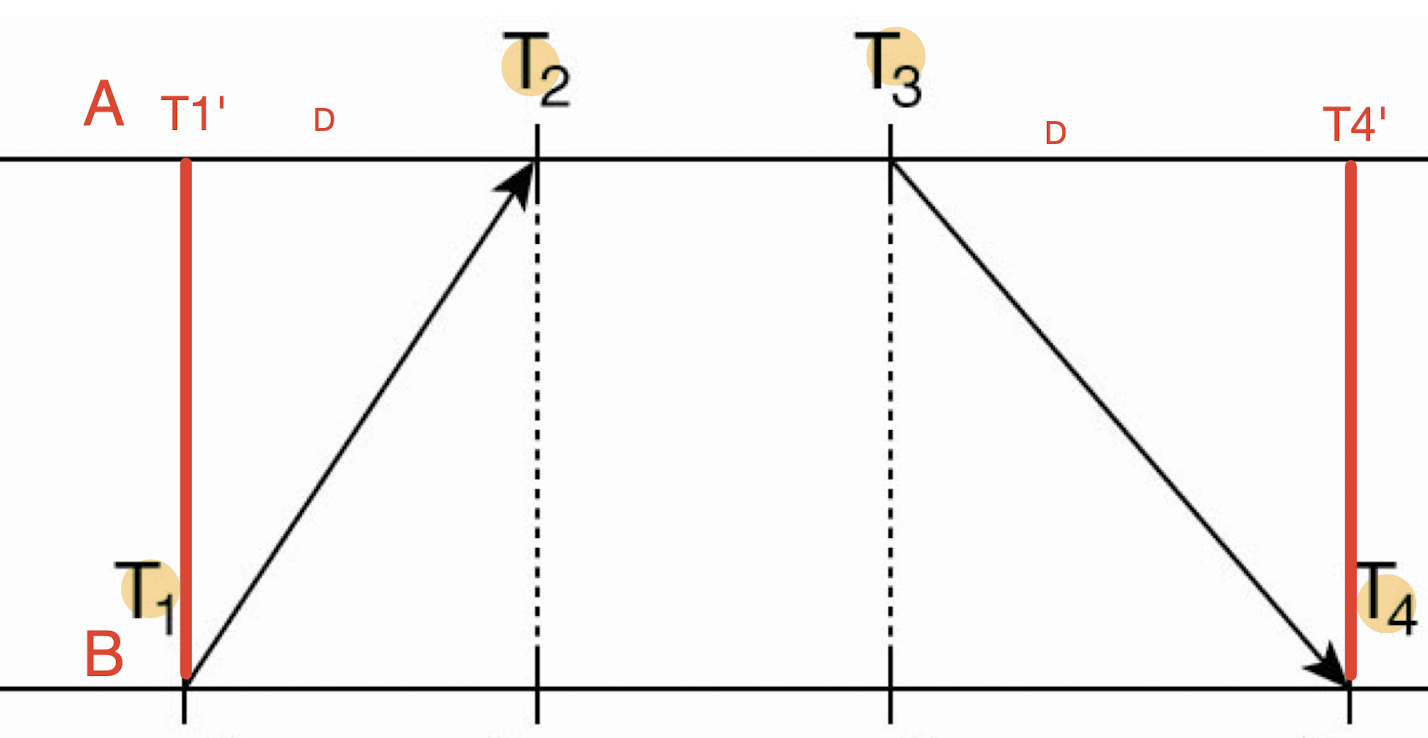
\includegraphics[width=\linewidth/4]{Q1.png}
\end{figure}

	
%Then, when calculating the round trip time \texttt{RTT}, time might be different on machine A and B. Thus, \underline{it must be calculated as $(T4 - T1) + (T3 - T2)$}, as $(T4-T1)$ is the total round trip time including the time machine A spent to formulate a response, and $(T3 - T2)$ is the time that machine A spent to formulate a response, and the subtraction between timestamp on the from the same machine ensured that it's the actual time, as that subtraction 'cancels out' the difference between the machine's time to the real time.
	
%Then, since we assumed the network delay from A to B is the same as the network delay from B to A, so we can calculate the \underline{\textbf{network delay} (D) as $\frac{RTT}{2} = \frac{(T4 - T1) + (T3 - T2)}{2}$}.
	
For the calculation of the \textbf{clock offset} ($\theta$), let's first introduce a variable \textbf{network delay} (D) (as the delay is same on both way, under the assumption). Then consider the an imaginary timestamp \texttt{T1'}, which is the current timestamp of machine A when machine B records it's current timestamp \texttt{T1}, and \texttt{T4'}, which is the current timestamp of machine B when machine A records it's current timestamp \texttt{T4}. Then, our $\theta$ should be $T1' - T1 = T4' - T4$.

With the above definition, we can write $T1' = \theta + T1$ and $T4' = \theta + T4$. From there, we can express $T2 = T1' + D = \theta + T1 + D$, which gives us $\theta = -D + T2 - T1$; And $T3 + D = T4'$ (as $T4'$ is the current timestamp of machine A when B records T4, so the time difference between $T3$ and $T4'$ should just be the network delay $D$), which gives us $T3 + D = \theta + T4$, which gives us $\theta = D + T3 - T4$.

Then, we add these two terms together to cancel out D, and thus we get the skew formula \underline{$\theta = \frac{T2-T1+T3-T4}{2}$}.

	
%Also, under the same assumption, we can calculate the \textbf{clock offset} ($\theta$) as $\frac{(T2 - T1) + (T3 - T4)}{2}$, as the difference between two machine's clock can be considered constant during the time we formulate this timestamp exchange, so the addition of a difference in timestamp of machine B to machine A and a difference in timestamp of machine A to machine B (I.E, the portion $(T2 - T1) + (T3 - T4)$) 'cancels out' the network delay between two machines

Then, we can just simply advance the time of machine B by $\theta$ (if $\theta <0$, then retreat time of machine B by $|\theta|$). Now we have synchronized the clock of machine B match that of machine A.

\newpage
%%%%%%%%%%%%%%%%%%%%%%%%%%%%%%%%%%%%%%%%%%%%%
%%%%%%%%%%%%%%%%%%%%%%%%%%%%%%%%%%%%%%%%%%%%%
\subsection{(3 mark)}
What is the Precision Time Protocol (PTP)? and why is it more accurate than the Network Time Protocol (NTP)? (not in slides, google to learn about PTP)\\

Precision Time Protocol (PTP) is a protocol defined in the IEEE 1588 standard, and is designed for precisely synchronize the clocks in distributed system (networked), and is able to achieve highly precise time synchronization (sub-microsecond in LAN).

Its main idea is to select a master clock from the clocks in the network and let all other clock (slave clocks) synchronize to it. The selection of the master clock is based on the clock's ability to produce the most accurate time (determined through predefined priorities, clock accuracy and network path's quality etc.).

Reasons why PTP is more accurate than NTP include but not limit to:

\begin{itemize}
	\item Hardware Time-stamping: \\ NTP usually relies on software time-stamping, and PTP uses hardware-supported time-stamping, which is not subject to delays and discrepancies introduced by software-level factors like the scheduling of operation system.
	
	\item Protocol Design: \\ NTP uses a generic hierarchical system for distributing time information across a wide range of environments (not designed specifically for achieving the highest possible precision), and PTP employed a master-slave architecture specifically designed for precision, which included algorithm like Best Master Clock Algorithm (BMCA) for selecting the most accurate clock (master clock) and other protocols for measuring and compensating for delays introduced by the networking.
	
	\item Delay Compensation: \\ NTP uses RTT to estimate network delays (assume same on both direction), and PTP employs both one-way and two-way delay measurement algorithm to accurately determine the delay and compensate for it.
	
\end{itemize}

\newpage
%%%%%%%%%%%%%%%%%%%%%%%%%%%%%%%%%%%%%%%%%%%%%
%%%%%%%%%%%%%%%%%%%%%%%%%%%%%%%%%%%%%%%%%%%%%
\subsection{(3 mark)}
How Causal ordered multicast can tolerate message reordering in the network. Meaning if server 1 sends message A then B to server 2, but due to message reordering in the network, server 2 receives message B first then A. How Causal ordered multicast can tolerate this reordering? \\

Firstly, Causal-ordered multicast ensures all nodes keeps a vector clock containing counters for all nodes, and the sender increment the counter for itself on its vector clock on message send, and send the message along side with its own versions of vector clock.

Then, all nodes buffers all received messages until the counter of the sender in the vector clock inside the message is one more than the counter of the sender stored locally (which ensured that when it processes this message from the sender, it didn't miss any message previously sent by the sender), and all other node's counter in the vector clock inside the message is less than or equal to the counter for these nodes stored locally (which ensured that when it processes this message from the sender, it didn't miss any previous message sent by node other than the sender).

And for any receiver, only increment the counter locally for the sender when the counter for the sender inside the message is one greater than the local counter for that sender (as sender only increment its own counter stored locally when sending its message, so the counter for the sender in the subsequent message sent by the sender is the same as the counter that the receiver have locally for the sender).

The outlined algorithm for comparing using the vector clock and the updating of vector clocks ensured any message received by any sender is processed by the receiver with the same 'context' (previously received message from any node) as the sender, which allows causal-ordered multicast to tolerate the reordering in the network.

\newpage
%%%%%%%%%%%%%%%%%%%%%%%%%%%%%%%%%%%%%%%%%%%%%
%%%%%%%%%%%%%%%%%%%%%%%%%%%%%%%%%%%%%%%%%%%%%
\subsection{(6 mark)}
Consider three processes executing the statements shown below. Assume that a, x, y, and z are initially 0. What are the possible values for a that can result from a sequentially consistent interleaving of the statements of the three processes? For each value of a, show one sequentially consistent interleaving yielding that value.

Process A

A1 : x = 1

A2 : if (y == 0) a = a + 1

Process B

B1 : y = 1

B2 : if (z == 0) a = a + 1

Process C

C1 : z = 1

C2 : if (x == 0) a = a + 1\\

Before all, since we have 3 \texttt{if} statement of incrementing $a$, which is initially 0, so the range of a is $0, 1, 2, 3$ (if condition is true or not yields only these 4 possibilities).

Firstly, we can very safe to say that it's not possible for $a$ to be $3$. Because once a process executes its first statement setting $x$, $y$, or $z$ to 1, the condition in another process that checks if the variable is 0 will be false.

For $a = 2$, one possible sequentially consistent interleaving of operations is $A1 \to A2 \to B1 \to B2 \to C1 \to C2$.

For $a = 1$, one possible sequentially consistent interleaving of operations is $A1 \to A2 \to B1 \to C1 \to B2 \to C2$.

For $a = 0$, one possible sequentially consistent interleaving of operations is $A1 \to B1 \to C1 \to A2 \to B2 \to C2$.


\newpage
%%%%%%%%%%%%%%%%%%%%%%%%%%%%%%%%%%%%%%%%%%%%%
%%%%%%%%%%%%%%%%%%%%%%%%%%%%%%%%%%%%%%%%%%%%%
\subsection{(6 mark)}
One problem with the 2PC protocol is that it may block under failures. To address this deficiency, three-phase commit (3PC) was proposed.

\begin{enumerate}
	\item[a] Describe a scenario in which 2PC will block? i.e., why it is not safe for participants to proceed with either abort or commit?\\
	
	One possible scenario is if the coordinator sends the prepare request then fail before sending commit or abort message based on participants' vote. 
	
	In this case, the participants cannot commit because they don't know if every participant has vote to commit. So if any participants commit and not all participant has vote to commit, it would violate the sequentially consistency assumption of the 2PC model.
	
	Also, the participants cannot abort because the decision to abort or commit must be coordinated. So if any participants commit and all other participants actually vote to commit, it would also violate the sequentially consistency assumption of the 2PC model.
	
	\item[b] How 3PC avoids this blocking case? (Hint: extra material, not in the slides, check the text book)\\
	
	3PC avoids this blocking case by adding an extra pre-commit phase, where the coordinator signal all participants that everyone agreed to commit if all participants vote to commit, then signalling all participants to actually commit after all participants acknowledged the pre-commit message.
	
	%This additional phase only before the signalling of commit for all participants ensures all participants are informed of the imminent commit that allows them to decide to commit even if the coordinator fails before the final commit phase. So, in the case mentioned above, all participants that votes commits can unilaterally decide to abort after not heard from the coordinator for a period of time rather than waiting indefinitely until the coordinator is back or an administrator intervene, thus keeps the sequentially consistency assumption of the 2PC model without blocking.
	
	With this additional stage, when a participant times out while waiting for a message from the coordinator, it means that the coordinator must have failed (or it is perceived as a coordinator failure). In this case, the participant initiates an election protocol to determine a new coordinator. Once a new coordinator is elected, the participants exchange status information about the transaction. If the new coordinator finds the transaction in at least a pre-commit state at any participant, it commits (in its local log) the transaction (as it would mean the previous coordinator decided to enter pre-commit stage, meaning all participants voted to commit); otherwise, it aborts the transaction. Then, this new coordinator proceeds to complete the 3PC for the transaction in all the other participants. If the new coordinator fails, the election process is repeated again.\footnote{"Three-Phase Commit." Encyclopedia of Database Systems (2009): 3091-3097. Web.}

	
\end{enumerate}


\newpage
%%%%%%%%%%%%%%%%%%%%%%%%%%%%%%%%%%%%%%%%%%%%%
%%%%%%%%%%%%%%%%%%%%%%%%%%%%%%%%%%%%%%%%%%%%%
\subsection{(6 mark)}
Each figure below shows a possible log configuration for a Raft server (the contents of log
entries are not shown; just their indexes and terms). Considering each log in isolation, could that
log configuration occur in a proper implementation of Raft? If the answer is "no," explain why
not.
\begin{enumerate}
	\item[a])\\ 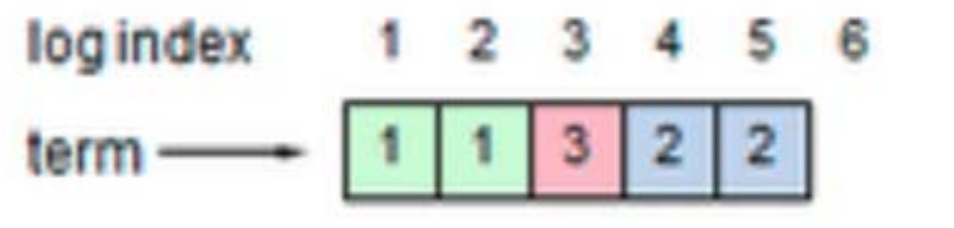
\includegraphics[width=\linewidth/3]{q6a.png}
	
	This is not possible because each server stores a \textit{current term} number, which increases monotonically over time. And if a server receives a request with a stale term number, it will reject the request.
	
	So there is no chance log 4 has a smaller term number than log 3, as this server would have reject log 4 and log 5 with term number 2.
	
	\item[b])\\ 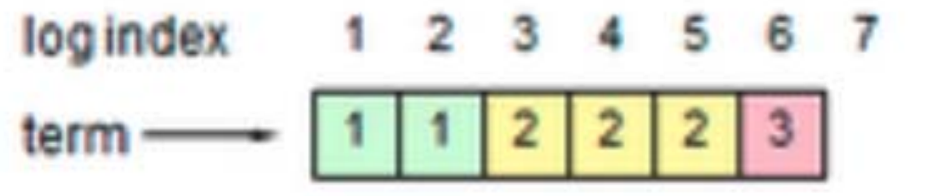
\includegraphics[width=\linewidth/3]{q6b.png}
	
	Yes.
	
	\item[c])\\ 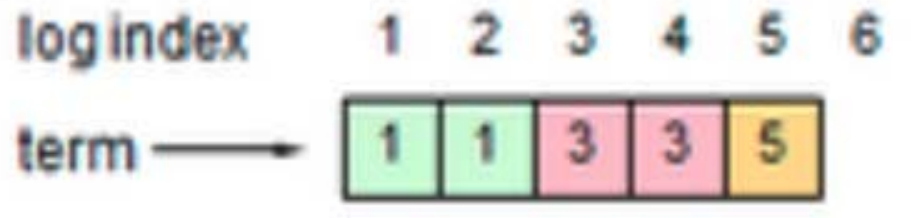
\includegraphics[width=\linewidth/3]{q6c.png}
	
	Yes.
	
\end{enumerate}

\newpage
%%%%%%%%%%%%%%%%%%%%%%%%%%%%%%%%%%%%%%%%%%%%%
%%%%%%%%%%%%%%%%%%%%%%%%%%%%%%%%%%%%%%%%%%%%%
\subsection{(3 mark)}
In Raft, suppose that a hardware or software error corrupts the nextIndex value stored by the leader for a particular follower. Could this compromise the safety of the system? Explain your answer.\\

No, this will not compromise the safety of the system. Let's assume the \texttt{nextIndex} value stored by the leader for a particular follower is $x$, and:
\begin{itemize}
	\item If \texttt{nextIndex} become larger than $x$:
	\subitem Then without considering any other safety mechanism, the \textbf{AppendEntries}'s consistency check will fail in the next \textbf{AppendEntries} RPC, then the leader will decrements \texttt{nextIndex} and attempt again. Eventually nextIndex will reach a point where the leader and follower's log will match.
	
	So, even if \texttt{nextIndex} become larger than the one plus the latest log of the leader itself, this mechanism alone is able to fix \texttt{nextIndex} because the last entry that the leader and followers log match is not possible for any entry leader has not saved yet. Thus keeping the system's safety.

	\item If \texttt{nextIndex} become smaller than $x$:
	\subitem Then without considering any other safety mechanism, the \textbf{AppendEntries} will succeed and starts to re-write this follower's log to match what log leader has starting from the now smaller \texttt{nextIndex}. It will not compromise the safety of the system as well.


\end{itemize}

\newpage
%%%%%%%%%%%%%%%%%%%%%%%%%%%%%%%%%%%%%%%%%%%%%
%%%%%%%%%%%%%%%%%%%%%%%%%%%%%%%%%%%%%%%%%%%%%
\subsection{(4 mark)}
In Raft, if a new configuration removes nodes from a cluster, the removed nodes will not receive heartbeats from the leader and may start leader election process and send RequestVote RPCs potentially with high term numbers. Such RequestVote RPCs will make the current leader step down and join the leader election process.
\begin{enumerate}
	\item[a] If this happens, can this affect the safety of the protocol? Why?
	
	Firstly, let's assume that this could happens (this cannot). Then, it would mean that the leader for previous term cannot be one of the removed nodes, as the leader would write the configuration change as an entry into its own log first, so it cannot 'not receiving'  this configuration change and keep electing for leader. 
	
	
	Then, these removed nodes will send RequestVote RPCs with new term numbers, which cause the current leader to revert to follower state. But these nodes will not become leaders, as they misses the configuration change log. Eventually a new leader will be elected, but the removed nodes will time out again and the entire process will repeat. This will not affect the safety of the protocol, but it will resulting in poor availability of the system.
	
	%Then this will affect the safety of the protocol, as the new configuration is stored and communicated as a special entry inside the log, since the removed nodes elected and become the leader, it must missed this configuration entry (otherwise it would step down and removed itself). So, if any new client requests goes into this node as its the leader, it would overwrite the configuration entry with the new client request in the same index, thus violates the \textbf{State Machine Safety} properties of the Raft. Which specifies that "if a server has applied a log entry at a given index to its state machine, no other server will ever apply a different log entry for the same index".
	
	\item[b] What is Raft's solution to avoid unnecessary runs of the leader election protocol?
	
	Raft avoids \textbf{unnecessary runs for the leader election protocol} by the rule that "servers disregard RequestVoteRPCs when they believe a current leader exists". To be more precisely, if a server receives a RequestVote RPC from other node within the minimum election timeout period of hearing from the current leader, it doesn't update its term nor vote.
	
	This way,  the removed servers will not be able to disrupt the cluster at all assuming the cluster is able to receive heartbeats from the leader. (removed server cannot become the leader is also ensured by having the rule that servers will not elect leader who has less term or have the same term but with less entry. Note the configuration change as an entry in the log, and if removed server attempt to become the leader, means it must have missed that entry, resulting in having less entry than server received the configuration change in the current term.)
	
\end{enumerate}


\newpage
%%%%%%%%%%%%%%%%%%%%%%%%%%%%%%%%%%%%%%%%%%%%%
%%%%%%%%%%%%%%%%%%%%%%%%%%%%%%%%%%%%%%%%%%%%%
\subsection{(4 mark)}
\begin{enumerate}
	\item[a] What are Merkle trees?
	
	Merkle tree is a data structure named after its proposer Ralph Merkel. It's an authenticated binary search tree based on a set of ordered values $x_1, x_2, \dots, x_n$. Where leaves corresponded to the ordered elements in the sets and contain the hash value of its elements. A leaf node associated with element $x_i$ contains the value $h(x_i)$, where $h()$ is a cryptographic one-way hash function, such as MD5 or SHA-1. Each internal node will have the corresponding hash value of the concatenation of its children (maintaining their order). For example, an internal node with children $v_1, v_2$ will have value $h(v_1 || v_2)$. Lastly, the root node is digitally signed.\footnote{Mykletun, Einar, Maithili Narasimha, and Gene Tsudik. "Providing authentication and integrity in outsourced databases using merkle hash trees." UCI-SCONCE Technical Report (2003).}
	
	\item[b] How Merkle trees are used in Dynamo?
	
	Dynamo uses Merkle trees to detect the inconsistencies between replicas faster and to minimize amount to transferred data. \footnote{DeCandia, Giuseppe et al. "Dynamo." ACM SIGOPS Operating Systems Review 41.6 (2007): 205-220. Web. }
	
	\item[c] What is the advantage and disadvantage of this approach?
	
	The advantage of this approach is that each branch of the tree can be checked independently without requiring nodes to download the entire tree or the entire dataset. Also, the use of Merkle trees help in reducing the amount of data that needs to be transferred while checking for inconsistencies among replicas. For example, if the hash values of the root of two trees are equal, then the values of the leaf nodes in the tree are equal and the nodes requires no synchronization. If not, it implies that the values of some replicas are different. In such cases, the nodes may exchange the hash values of children and the process continues until it reaches the leaves of the trees, at which point the hosts can identify the keys that are "out of sync". Merkle trees minimize the amount of data that needs to be transferred for synchronization and reduce the number of disk reads performed during the anti-entropy process. \footnotemark[\value{footnote}] 
	
	The disadvantage of this approach is that many key ranges change when a node joins or leaves the system thereby requiring the tree(s) to be recalculated.\footnotemark[\value{footnote}]
	
\end{enumerate}

\newpage
%%%%%%%%%%%%%%%%%%%%%%%%%%%%%%%%%%%%%%%%%%%%%
%%%%%%%%%%%%%%%%%%%%%%%%%%%%%%%%%%%%%%%%%%%%%
\end{document}
